\documentclass[10pt,journal]{IEEEtran}
%\IEEEoverridecommandlockouts

\usepackage[spanish,es-tabla]{babel} % Idioma español con tablas
\usepackage[spanish]{babel}
\usepackage[table,xcdraw]{xcolor} % Para pintar tablas
\usepackage{url} % Para colocar URL
\usepackage{amsmath,amssymb,amsfonts}
\usepackage{graphicx}
\usepackage{textcomp}
\usepackage{xcolor}
\usepackage{float} % Para var H, figure

\usepackage[square,numbers]{natbib}
\bibliographystyle{abbrvnat}

\renewcommand{\baselinestretch}{1.5}     %interlineado

\title{Dispositivos de Almacenamiento Actuales y sus Aplicaciones}

\author{
\IEEEauthorblockN{{\Large Angely Mendez Cruz}} \\
\vspace{2mm}
\IEEEauthorblockA{\textit{Organización de Archivos} \\
\textit{Escuela de Informática} \\
\textit{Facultad de Ciencias Físicas y Matemáticas} \\
\textit{Universidad Nacional de Trujillo, \\ Perú }
\\ \vspace{1mm}
t052701020@unitru.edu.pe}}

\begin{document}

\maketitle

    \begin{abstract}
    En este trabajo de investigación se brinda información, respecto al
    al almacenamiento, es decir a sus dispositivos, los que actualmente siguen siendo usados, en adición, a aquellas nuevas formas de guardar datos en la red y/o la nube, teniendo varios ejemplos habilitados a nivel mundial de servidores, computadoras y/o discos duros, de tal manera que los datos que se almacenen allí permanezcan accesibles a todos los usuarios con acceso a dicha red, de este modo se conforma un sistema de grande capacidad de almacenar.
    \end{abstract}
    
    \section{\textbf{Introducción}}
    
    En la actualidad y ante la evolución de los dispositivos de almacenamiento, la generación y mejoras de estos sigue incrementando. Las tecnologías cambian y con ellas la gestión documental también; los dispositivos de almacenamiento masivo se convierten en una ventaja  para el manejo de diferentes archivos masivos actuales que custodian no solo fuentes, documentos en soporte físico, sino también en soporte electrónico.
    
    Además, mucha información debe intercambiarse entre distintos equipos. Aparte de las redes informáticas (incluida Internet), este problema hace necesario contar con unidades de discos o cintas intercambiables, o usar unidades removibles, es decir, que pueden extraerse completas de un equipo para conectarlas a otro.
    
    En cuanto a las unidades externas, que se conectan al ordenador por medio de un puerto exterior (serie, paralelo o USB), también son intercambiables entre distintos equipos.
    
    Pero como anteriormente se mencionó, surge un problema que se debe considerar, la capacidad. Por lo que, conforme la tecnología avanza, más datos se van generando, y es necesario contar con un almacenamiento eficiente para poder guardar toda esa información y acceder a ellos.

    \section{\textbf{Almacenamiento de Datos}}
    \subsection{\textbf{Definición}}
    El \textbf{almacenamiento de datos} es el proceso tecnológico por el cual se archiva, organiza y comparten \textit{los bytes de información} que componen los archivos que se utilizan en el día a día como: 
    \begin{enumerate}
        \item Documentos de texto.
        \item Imágenes, vídeos, configuraciones.
        \item Sonidos y cualquier otra información en formato digital \citep{guevara2016implementacion}.
    \end{enumerate}
    
    
    El \textbf{cambio ha ido en aumento} de estos dispositivos desde los primeros sistemas de disco magnéticos, que muy probablemente se sigan utilizando pero no con mucha frecuencia, sin embargo actualmente existe una forma más digital de almacenar datos por ejemplo: \textit{hoy se encuentran conectados a una red} o pueden estar son definidos por un software.
    
    El almacenamiento de datos tiene un \textbf{proceso a través del uso de la tecnología, ésta se aplica para organizar, distribuir y archivar información con los bytes y los bits} que son parte de los sistemas de los que la gente depende día con día, llega a ser tan importante en todos los servicios: desde una simple aplicación, contenido multimedia, direcciones, contactos, hasta protocolos de red y todo lo que tiene que ver con el mundo digital.

    Para \textbf{Andrea Cubillos}, Ex Gerente Comercial Colombia, Hitachi Data Systems en una entrevista en 2009, considera que el manejo adecuado de las tecnologías de almacenamiento de acuerdo con el valor de la información en el tiempo; \textit{"desde el punto de vista de la administración es el pilar en una empresa tecnológica"} \citep{RevistaS75:online}, porque implica costos del almacenamiento.
    
    Respecto a esa opinión, desde aquellos años, observado desde una perspectiva empresarial y no solo tecnológica, la información y a su vez los medios de almacenamiento para guardar esa información tienen un valor diferente en el tiempo. Siendo necesario ese sentido definir estrategias económicas de almacenamiento que les permita, a las empresas, clasificar la información de acuerdo con el valor de la misma en el medio de almacenamiento adecuados y más modernos.
    
    \subsection{\textbf{Características}}
    Además, dado que el almacenamiento de datos se realiza en dispositivos de hardware, disponen de unas características que los definen y que los hacen más adecuados para guardar copias de seguridad, dar acceso a los datos, transportar la información y otras funciones.
    
    Ellos cuentan con algunas principales características que los resaltan y son: 
    
    \begin{itemize}
        \item \textbf{Capacidad: }Mide la cantidad de datos que puede almacenar el sistema de almacenamiento, y es medida en \textit{bytes} (Gigabytes o Terabytes, habitualmente, aunque con el Big Data se manejan incluso Petabytes). 
    
        \item \textbf{Rendimiento: }Evalúa la rapidez y eficiencia en el sistema de almacenamiento de datos. 
        
        \item \textbf{Fiabilidad: }Es la disponibilidad de los datos cuando son solicitados, así como el hecho de disponer de una baja tasa de errores o fallos (por ejemplo, utilizando una configuración RAID). 
    
        \item \textbf{Recuperabilidad: }Mide la capacidad del sistema para recuperar datos tras una pérdida, borrado, corrupción o cualquier otro incidente que impida el acceso a los mismos.
    \end{itemize}
    
    \subsection{\textbf{Diferencia entre Almacenamiento y Memoria}}
    Generalmente los usuarios de computadoras consideran que la memoria y el almacenamiento son lo mismo.
    
    Sin embargo, aquellos usuarios que se dan cuenta que existe una diferencia entre las dos, frecuentemente no pueden identificar la diferencia \citep{Ladifere16:online}.
    
    A continuación, un cuadro comparativo, (Ver Tabla ~\ref{tab1} ) entre ellos:

    \begin{table}[H]
    \centering
    \caption{Almacenamiento y Memoria}
    \label{tab1}
    \begingroup
    \setlength{\tabcolsep}{5pt} % Default value: 6pt
    \renewcommand{\arraystretch}{1.1} % Default value: 1
    \begin{tabular}{|cc|lll}
    \cline{1-2}
    \multicolumn{2}{|c|}{\cellcolor[HTML]{000000}{\color[HTML]{FFFFFF} \begin{tabular}[c]{@{}c@{}}Diferencias entre Almacenamiento\\ y Memoria\end{tabular}}}                                                                                                                                          &  &  &  \\ \cline{1-2}
    \multicolumn{1}{|c|}{\cellcolor[HTML]{C0C0C0}{\color[HTML]{000000} Almacenamiento}}                                                                          & \cellcolor[HTML]{C0C0C0}{\color[HTML]{000000} Memoria}                                                                              &  &  &  \\ \cline{1-2}
    \multicolumn{1}{|c|}{{\color[HTML]{000000} \begin{tabular}[c]{@{}c@{}}Permite acceder a los \\ datos a largo \\ plazo.\end{tabular}}}                        & {\color[HTML]{000000} \begin{tabular}[c]{@{}c@{}}Permite acceder a los \\ datos en corto \\ plazo.\end{tabular}}                    &  &  &  \\ \cline{1-2}
    \multicolumn{1}{|c|}{{\color[HTML]{000000} \begin{tabular}[c]{@{}c@{}}Capacidad para \\ guardar aplicaciones, \\ SO por tiempo \\ indefinido.\end{tabular}}} & {\color[HTML]{000000} \begin{tabular}[c]{@{}c@{}}La velocidad del \\ computador y \\ rendimiento \\ dependen de             ella.\end{tabular}} &  &  &  \\ \cline{1-2}
    \end{tabular}
    \endgroup
    \end{table}

    
    \section{\textbf{Dispositivos de Almacenamiento Actuales}}
    
    Los dispositivos de almacenamiento son aquellos elementos de hardware que
    utilizamos para almacenar toda la información del ordenador tales como el 
    sistema operativo, nuestros archivos,programas, etc.

    A mediados de la década de 1970, cuando se dio la comercialización de dispositivos de almacenamiento de acceso directo o discos duros de IBM (International Business Machines Corp.), que implicaban una capacidad aproximada de 30 Megabytes; que si bien no era demasiado, sí era
    muy alto para aquel tiempo \cite{glossbrenner1993file}.
    
    Entonces, el alto costo y la necesidad de compartir y comunicar información entre usuarios obligaron a que los fabricantes y desarrolladores crearán nuevos dispositivos de almacenamiento.
    
    Su importancia en los equipos es vital pues en ellos está instalado o grabado todo 
    aquello que solicitemos al usar nuestro equipo. 
    
    \subsection{\textbf{Dispositivos magnéticos}}
    
    Un claro ejemplo de estos dispositivos, según Beekman \cite{george1999introduccion}, son los \textbf{\textit{discos magnéticos}}. La unidad de disco del computador puede recuperar información 
    rápidamente de cualquier parte del disco magnético, sin importar el orden en que fue grabada, de la misma forma que puede seleccionar casi al instante cualquier pista en un disco compacto (CD: compact disc).
    
    Todo ello, gracias a su \textbf{capacidad de acceso aleatorio}, estos discos son muy 
    populares en el mundo del almacenamiento de datos.
    
    Por ejemplo, un Disco Duro, (ver Figura  ~\ref{f2}), es un disco rígido, con sensibilidad magnética, que puede contener decenas o cientos de \textit{MEGABYTES} de información.
    
    \begin{figure}[H]
        \begin{center}
        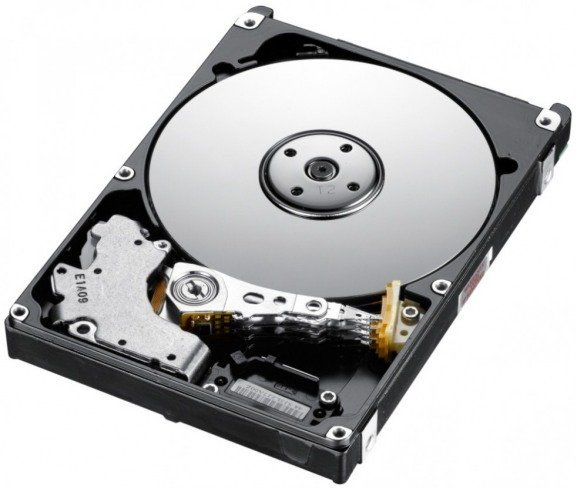
\includegraphics[width=0.25 \textwidth]{Discomagne.jpg}
        \caption{Disco Magnético - Disco Duro}
        \label{f2} 
        \end{center}
    \end{figure}
    
    \subsection{\textbf{Dispositivos ópticos}}
    
    Al aumentar la popularidad del multimedia, incluso un disco duro con gran capacidad
    se llenará rápidamente con sonidos, imágenes a color, secuencias de video y otros elementos que requieren gran cantidad de espacio de almacenamiento.
    
    Ante esta situación de incrementar más datos, es recomendable aplicar, \textbf{discos ópticos} son una alternativa más eficiente\cite{george1999introduccion}.
    
    Cabe resaltar que, una unidad de este disco usa rayos láser en lugar de imanes para leer y escribir información en la superficie del disco.
    
    Aunque no todos son muy rápidos como los disco duros, los disco ópticos tienen mucho más espacio para almacenar datos. Algunos los llaman \textit{"GIGABYTES"}.
    
    Las unidades de \textbf{CD-ROM}, Figura ~\ref{f3}, (compact disc-read-only memory), (disco compacto- memoria lectura), son unidades ópticas capaces de leer CD-ROM, discos de datos físicamente a un disco compacto musical.
    
    Como son unidades de sólo lectura, no pueden usarse como dispositivos de almacenamiento secundario.
    
    \begin{figure}[H]
        \begin{center}
            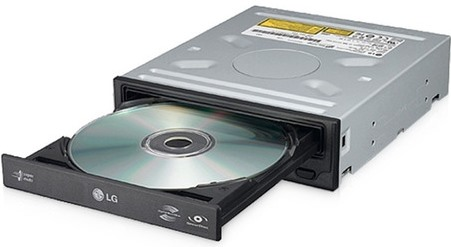
\includegraphics[width=0.3 \textwidth]{cd-rom.jpg}
            \caption{Disco Óptico - CD-ROM}
            \label{f3} 
        \end{center}
    \end{figure}

    \subsection{\textbf{Dispositivos digitales}}
    
    \subsubsection{\textbf{En la Red}}
    
    \begin{itemize}
    \item \underline{\textbf{Definición}}
    
    El desarrollo de la tecnología en almacenamiento sigue presentando nuevas formas como la
    PCM(Pulse Code Modulation), que de acuerdo con \cite{criptogr4:online},
    tiene la facultad de \textit{facilidad de integración, escalabilidad, velocidad y resistencia}; esta podría ser una opción en un sistema de almacenamiento de grandes capacidades de datos.
    
    Además, sus bondades prometen ser memorias no volátiles de próxima generación \cite{yoon2013integrated}, considerando que muchas aplicaciones modernas exigen cada vez más para el \textbf{manejo de grandes cantidades de datos}. 
    
    Las redes han evolucionado con el paso del tiempo y en la actualidad una \textit{\textbf{red empresarial}} tiene una capacidad de transferencia de al menos 1000 Mbps (en caso de red de fibra óptica, de 10 Gbps), lo que permite transferir mucha información en poco tiempo.
    
    Esta velocidad de transferencia ha hecho populares métodos de almacenamiento en red como SAN \textit{(cuyo uso principal es en servidores de aplicaciones)} o NAS \textit{(destinados sobre todo a almacenamiento empresarial o personal)}.
    
    \item \underline{\textbf{Clasificación}}
    
    El almacenamiento de datos se puede clasificar, Figura ~\ref{f1}, desde el punto de las estructuras de sistemas de 
    almacenamiento con opciones como:
    
    \begin{itemize}
    \item \textbf{DAS} (Direct Attached Storage o Almacenamiento de Conexión Directa).
    \item \textbf{NAS} (Network Attached Storage o Almacenamiento Conectado en Red).
    \item \textbf{SAN} (Storage Area Network o Red de área de Almacenamiento).
    \item \textbf{Sistemas de almacenamiento en la nube}, que incluye capacidades de espacio en unidades de discos 
    duros tradicionales y sólidos, así como la tecnología de la Memoria de Cambio de Fase (PCM: Phase Change Memory).
    \end{itemize}
    
    \begin{figure}[H]
        \begin{center}
            \includegraphics[width=0.47 \textwidth]{Clasificación.png}
            \caption{Clasificación del almacenamiento de datos o Data Storage.}
            \label{f1} 
        \end{center}
    \end{figure}
    
    \item \underline{\textbf{En la Nube}}
    
    El almacenamiento de datos en la nube, también llamado \textit{cloud computing}, se da gracias al uso de equipos virtuales; para los cuáles se necesita una infraestructura informática invisible para el usuario, pero al utilizarla parece que se tuviera un equipo físico real.
    
    De esta manera, la gran ventaja se puede determinar en \textbf{el número de procesamiento, el sistema operativo, el tamaño de memoria RAM y de disco de almacenamiento}.
    
    Esta elasticidad en la infraestructura es una de las técnicas usables en \textit{\textbf{Big data}} donde las tecnologías de virtualización han hecho que la computación sea \textit{accesible, asequible y rentable}.
    
    Una gran beneficio de los entornos de la nube es que, sin duda, proporciona una posible herramienta para el almacenamiento de grandes volúmenes de datos.
    
    En este espacio para \textbf{acopiar datos, información, objetos digitales, y otros,} que se acceden por internet a través de un servicio web, mediante un navegador como \textbf{Explorer, Firefox, Chrome o Safari}.
    
    Además de un aprovisionamiento de recursos informáticos bajo demanda, con control variable para el usuario y neutrales ante sistemas operativos \cite{vazquez2015tecnologias}, estas características hacen único al almacenamiento en la nube.
    
    Teniendo en cuenta que el almacenamiento puede ser brindado por un proveedor de servicios \textit{\textbf{(nube pública)}} o una versión privada \textit{\textbf{(nube privada)}}; esta última es creada por una organización particular para su uso interno, con un completo control de los recursos en tecnologías de información.
    
    A continuación algunos \textbf{proveedores de servicios de almacenamiento en la nube}, Figura ~\ref{f4}:
    
    \begin{enumerate}
        \item {\large \textbf{Amazon}} \\
        Es una de los principales proveedores de servicios en la nube y, además de su eficiencia, presenta mejor garantía de servicio.
        
        El servicio de \textit{Amazon Simple Storage Service (Amazon S3)} es una interfaz de servicios web que puede utilizarse para almacenar y recuperar grandes cantidades de datos, en cualquier momento y desde cualquier parte de la web.
        \item {\large \textbf{IBM}} \\
        Los servicios de cloud computing de IBM incluyen también el almacenamiento con \textit{IBM Smart Business Storage Cloud}, permitiendo que los usuarios tengan un acceso eficiente, rentable y experimenten una disminución del rendimiento e interrupciones.
        \item {\large \textbf{Google}} \\
        Siendo un gigante de la industria de la informática ofrece servicios a través de \textit{Google App Engine}, que es una plataforma que ofrece construcción y alojamiento de aplicaciones web con la infraestructura de Google, donde solo se paga lo que se utiliza.
        
        Permite que los recursos informáticos sean fáciles de construir, mantener y escalar a medida que crecen las necesidades de almacenamiento y tráfico de web.
    \end{enumerate}
    
    \begin{figure}[H]
        \begin{center}
            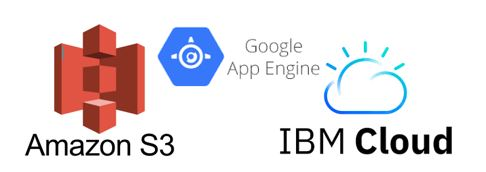
\includegraphics[width=0.5 \textwidth]{logos.JPG}
            \caption{Logos Proveedores de Almacenamiento en la Nube}
            \label{f4} 
        \end{center}
    \end{figure}
    \end{itemize}
    
    \section{\textbf{Aplicaciones de los Dispositivos de Almacenamiento Actuales}}
    
    \begin{itemize}
    \item \underline{\textbf{Almacenamiento de Conexión Directa (DAS)}} \\
    El entorno de uso de este tipo de arquitectura de almacenamiento es ideal para el intercambio de archivos localizados en ambientes con \textbf{un único servidor o unos cuantos servidores}, Figura ~\ref{f5}.
    
    Por ejemplo, una pequeña biblioteca que no necesita compartir información a través de largas distancias.
    Naturalmente se convierte en la elección previa para las pequeñas unidades de información, debido a que cuentan con \textbf{menos recursos financieros}.
    
    Principalmente es utilizado en las \textbf{computadoras personales y pequeños servidores}, que soportan solo aplicaciones que requieren capacidades bajas de almacenamiento y no admite directamente equipos múltiples de almacenamiento compartido.
    
    \begin{figure}[H]
        \begin{center}
            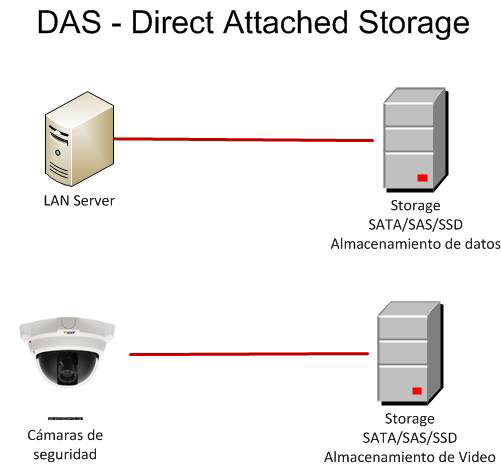
\includegraphics[width=0.3 \textwidth]{Das.png}
            \caption{ Método de Almacenamiento - DAS (Direct Attacked Storage)}
            \label{f5} 
        \end{center}
    \end{figure}
    
    \item \underline{\textbf{Discos duros para consolas}} \\
    Existen dos tipos de discos duros externos para consolas, los SSD, Figura ~\ref{f6}, y los HDD.
    Por un lado, los \textbf{SSD (unidades en estado sólido)}, son discos que no tienen partes mecánicas y su sistema de almacenamiento de archivos es en tarjetas flash conectadas entre sí. Mientras que los \textbf{HDD son los discos duros mecánicos}. La diferencia reside que, los SSD, son más caros, consumen menos, más rápidos y más silenciosos que los HDD, características necesarias para una consola de videojuegos.
    
    \begin{figure}[!htp]
        \begin{center}
            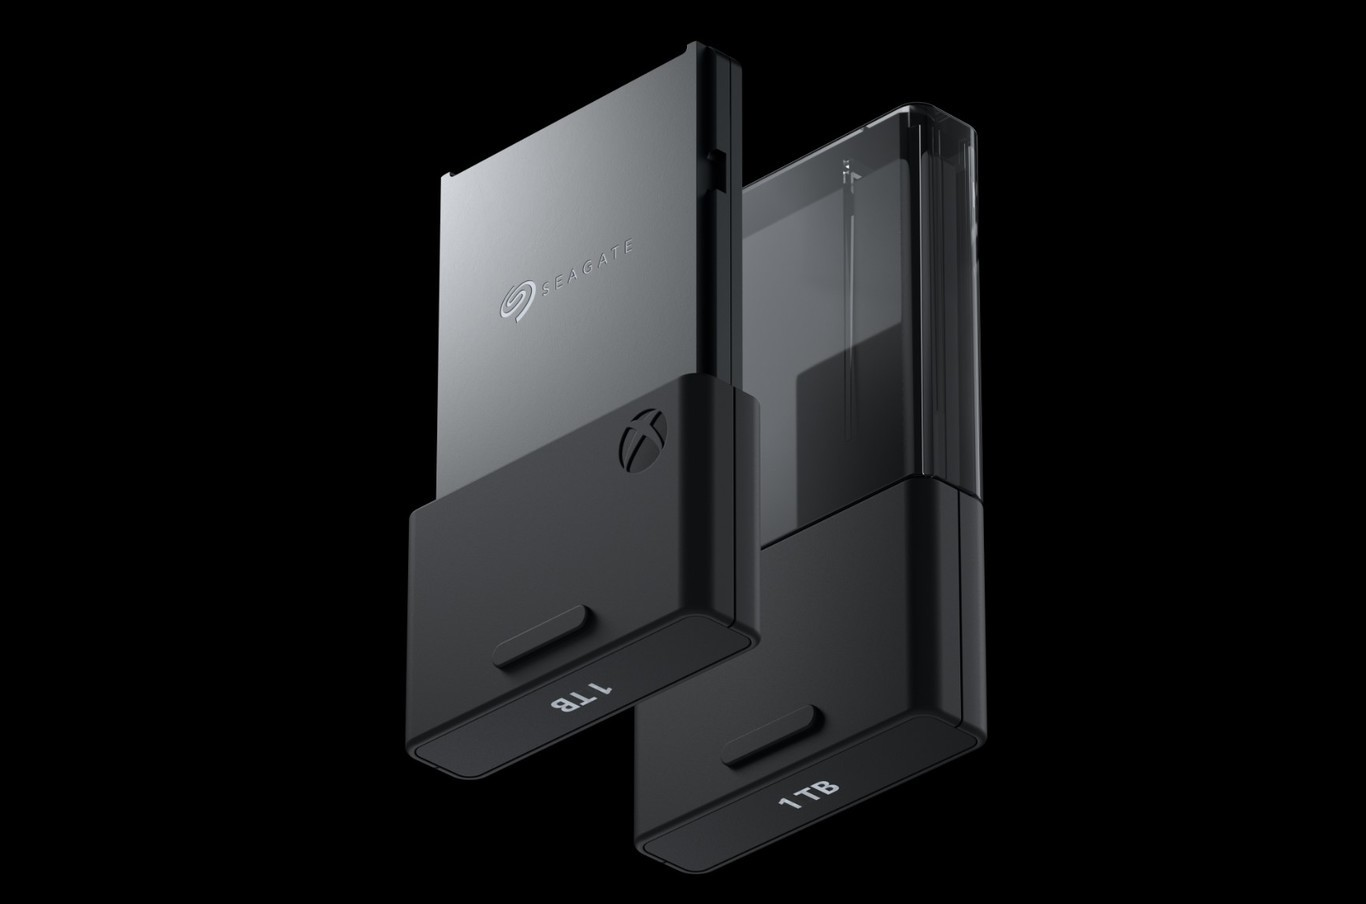
\includegraphics[width=0.4 \textwidth]{SSD.JPG}
            \caption{SSD para videojuego PS5}
            \label{f6} 
        \end{center}
    \end{figure}
    
    \item \underline{\textbf{Sistema bibliotecario}} \\
    En el sistema bibliotecario de la \textbf{Universidad Nacional Autónoma de México (UNAM)} cuentan con una arquitectura de almacenamiento del tipo SAN con fibra óptica, con un \textbf{espacio de 6TB} para la colección de fondo antiguo, mientras que el catálogo de Scielo México se conforma por 600GB.
    
    Otro dato interesante es la cantidad de espacio destinada para la colección de tesis, que se contempla en \textbf{700GB}.
    Por otra parte, el portal de revistas científicas y arbitradas de la UNAM \textbf{rebasa 700 GB,} considerando su base de datos y archivos, el cual sigue creciendo y pertenece a la infraestructura denominada “UNAM Cloud’’ \cite{RedalycT88:online}.
    \end{itemize}
    
    \section{\textbf{Conclusiones}}
    Es preciso decir que al pasar los años, desde el primer dispositivo de almacenamiento y el proceso que 
    involucra su evolución y la de otros dispositivos, las nuevas tecnologías han sido muy útiles para organizar, distribuir y almacenar grandes cantidades de datos e información, centrándose siempre en ser más eficientes.
    
    Por ello, es de suma relevancia en la actualidad, evaluar las diferentes opciones que existen para almacenar nuestra información o de la empresa a la que pertenecemos, tomando en cuenta, la capacidad que necesitamos para almacenar nuestros datos, además del del rendimiento y el costo que involucra.
    
    Finalmente, las grandes unidades de información que tienen mayores presupuestos y requerimientos altos de transferencia y transmisión de datos, son beneficiados ante la oferta de las nubes, la virtualización y las redes de almacenamiento, permitiéndoles la reducción de costos y la expansión de la capacidad, lo que produce una adecuada gestión de las informaciones.
\medskip
\bibliography{Referencia}

\end{document}
